%9_Gauss_distribution
%notes for the course Probability and Statistics COMS10011
%taught at the University of Bristol
%2018_19 Conor Houghton conor.houghton@bristol.ac.uk
%To the extent possible under law, the author has dedicated all copyright
%and related and neighboring rights to these notes to the public domain 
%worldwide. These notes are distributed without any warranty. 

\documentclass[11pt,a4paper]{scrartcl}
\typearea{12}
\usepackage{graphicx}
%\usepackage{pstricks}
\usepackage{listings}
\usepackage{color}

\lstset{language=C}
\usepackage{fancyhdr}
\pagestyle{fancy}
\lfoot{\texttt{github.com/COMS10011/2018\_19}}
\lhead{COMS100011 9\_Gauss\_distribution - Conor}
\begin{document}

\section*{9 The Gau\ss{}ian distribtion}

The Gau\ss\footnote{\ss{} is a German letter equivalent to ss} or Gauss
or normal or Gau\ss{}ian or Gaussian or bell-curve distribution is a
continuous distribution which is used to model a whole range of
natural phenomenon, in fact, much of statistics and almost all
statistics outside of science, assumes almost everything has a
Gau\ss{}ian distribution. We will see why later on, basically there is
a theorem, the Central Limit Theorem, that tells us why the
Gau\ss{}ian distribution is as common as it is. For now though we will
look at the distribution and its properties.

\begin{figure}[tb]
\begin{center}
% GNUPLOT: LaTeX picture with Postscript
\begingroup
  \makeatletter
  \providecommand\color[2][]{%
    \GenericError{(gnuplot) \space\space\space\@spaces}{%
      Package color not loaded in conjunction with
      terminal option `colourtext'%
    }{See the gnuplot documentation for explanation.%
    }{Either use 'blacktext' in gnuplot or load the package
      color.sty in LaTeX.}%
    \renewcommand\color[2][]{}%
  }%
  \providecommand\includegraphics[2][]{%
    \GenericError{(gnuplot) \space\space\space\@spaces}{%
      Package graphicx or graphics not loaded%
    }{See the gnuplot documentation for explanation.%
    }{The gnuplot epslatex terminal needs graphicx.sty or graphics.sty.}%
    \renewcommand\includegraphics[2][]{}%
  }%
  \providecommand\rotatebox[2]{#2}%
  \@ifundefined{ifGPcolor}{%
    \newif\ifGPcolor
    \GPcolorfalse
  }{}%
  \@ifundefined{ifGPblacktext}{%
    \newif\ifGPblacktext
    \GPblacktexttrue
  }{}%
  % define a \g@addto@macro without @ in the name:
  \let\gplgaddtomacro\g@addto@macro
  % define empty templates for all commands taking text:
  \gdef\gplbacktext{}%
  \gdef\gplfronttext{}%
  \makeatother
  \ifGPblacktext
    % no textcolor at all
    \def\colorrgb#1{}%
    \def\colorgray#1{}%
  \else
    % gray or color?
    \ifGPcolor
      \def\colorrgb#1{\color[rgb]{#1}}%
      \def\colorgray#1{\color[gray]{#1}}%
      \expandafter\def\csname LTw\endcsname{\color{white}}%
      \expandafter\def\csname LTb\endcsname{\color{black}}%
      \expandafter\def\csname LTa\endcsname{\color{black}}%
      \expandafter\def\csname LT0\endcsname{\color[rgb]{1,0,0}}%
      \expandafter\def\csname LT1\endcsname{\color[rgb]{0,1,0}}%
      \expandafter\def\csname LT2\endcsname{\color[rgb]{0,0,1}}%
      \expandafter\def\csname LT3\endcsname{\color[rgb]{1,0,1}}%
      \expandafter\def\csname LT4\endcsname{\color[rgb]{0,1,1}}%
      \expandafter\def\csname LT5\endcsname{\color[rgb]{1,1,0}}%
      \expandafter\def\csname LT6\endcsname{\color[rgb]{0,0,0}}%
      \expandafter\def\csname LT7\endcsname{\color[rgb]{1,0.3,0}}%
      \expandafter\def\csname LT8\endcsname{\color[rgb]{0.5,0.5,0.5}}%
    \else
      % gray
      \def\colorrgb#1{\color{black}}%
      \def\colorgray#1{\color[gray]{#1}}%
      \expandafter\def\csname LTw\endcsname{\color{white}}%
      \expandafter\def\csname LTb\endcsname{\color{black}}%
      \expandafter\def\csname LTa\endcsname{\color{black}}%
      \expandafter\def\csname LT0\endcsname{\color{black}}%
      \expandafter\def\csname LT1\endcsname{\color{black}}%
      \expandafter\def\csname LT2\endcsname{\color{black}}%
      \expandafter\def\csname LT3\endcsname{\color{black}}%
      \expandafter\def\csname LT4\endcsname{\color{black}}%
      \expandafter\def\csname LT5\endcsname{\color{black}}%
      \expandafter\def\csname LT6\endcsname{\color{black}}%
      \expandafter\def\csname LT7\endcsname{\color{black}}%
      \expandafter\def\csname LT8\endcsname{\color{black}}%
    \fi
  \fi
  \setlength{\unitlength}{0.0500bp}%
  \begin{picture}(5040.00,3528.00)%
    \gplgaddtomacro\gplbacktext{%
      \csname LTb\endcsname%
      \put(858,440){\makebox(0,0)[r]{\strut{} 0}}%
      \put(858,793){\makebox(0,0)[r]{\strut{} 0.05}}%
      \put(858,1146){\makebox(0,0)[r]{\strut{} 0.1}}%
      \put(858,1499){\makebox(0,0)[r]{\strut{} 0.15}}%
      \put(858,1852){\makebox(0,0)[r]{\strut{} 0.2}}%
      \put(858,2204){\makebox(0,0)[r]{\strut{} 0.25}}%
      \put(858,2557){\makebox(0,0)[r]{\strut{} 0.3}}%
      \put(858,2910){\makebox(0,0)[r]{\strut{} 0.35}}%
      \put(858,3263){\makebox(0,0)[r]{\strut{} 0.4}}%
      \put(990,220){\makebox(0,0){\strut{}-4}}%
      \put(1447,220){\makebox(0,0){\strut{}-3}}%
      \put(1903,220){\makebox(0,0){\strut{}-2}}%
      \put(2360,220){\makebox(0,0){\strut{}-1}}%
      \put(2817,220){\makebox(0,0){\strut{} 0}}%
      \put(3273,220){\makebox(0,0){\strut{} 1}}%
      \put(3730,220){\makebox(0,0){\strut{} 2}}%
      \put(4186,220){\makebox(0,0){\strut{} 3}}%
      \put(4643,220){\makebox(0,0){\strut{} 4}}%
    }%
    \gplgaddtomacro\gplfronttext{%
    }%
    \gplbacktext
    \put(0,0){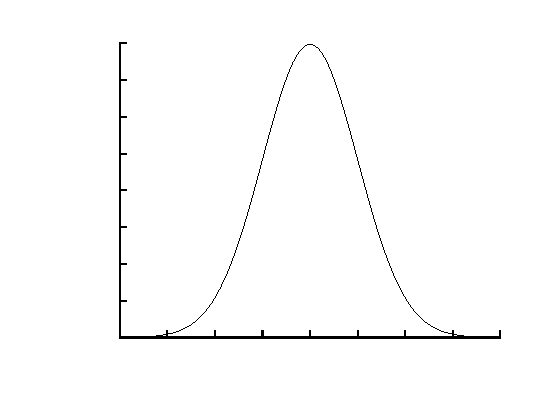
\includegraphics{fig_gauss}}%
    \gplfronttext
  \end{picture}%
\endgroup

\end{center}
\caption{A normal curve with mean zero and variance one.\label{fig_gauss}}
\end{figure}

The Gau\ss{}ian distribution with zero mean and unit variance is given by
\begin{equation}
p(x)=\frac{1}{\sqrt{2\pi}}e^{-x^2/2}
\end{equation}
It has a classic \lq{}bell\rq{} shape seen in Fig.~\ref{fig_gauss}; it
looks a bit like a binomial distribution with $p=0.5$. The slightly
confusing thing is the $1/\sqrt{2\pi}$, that is there to normalize the curve:
\begin{equation}
\int_{-\infty}^\infty e^{-x^2/2}dx=\sqrt{2\pi}
\end{equation}
This is confusing because we can do this definite integral, but the
corresponding indefinite integral can't be done in the sense that we
can't write down a formula in terms of functions we already
know. There is a trick for doing the definite integral which we won't
look at here for reasons of time but is very nice if you want to look
it up.

First lets work out the mean and variance of this distribution, it is
a maybe surprising thing that the integrals required for calculating
the mean and variance are much easier than the integral mentioned
above for normalizing the curve. So, mean first
\begin{equation}
\mu=\int_{-\infty}^\infty xp(x)dx =\frac{1}{\sqrt{2\pi}}\int_{-\infty}^\infty xe^{-x^2/2}dx
\end{equation}
This integral is very easy because the integrand is odd: a function $f(x)$ is odd if $f(-x)=-f(x)$. Now consider the integral from minus infinity to infinity of an odd function
\begin{equation}
\int_{-\infty}^\infty f(x)dx=\int_{-\infty}^0 f(x)dx+\int_0^\infty f(x)dx
\end{equation}
then let $x'=-x$ in the second integral. Note that $dx'=-dx$ and $x=\infty$ means $x'=-\infty$ and swithcing around the limits in an integral changes the sign:
\begin{equation}
\int_b^a g(x)dx=-\int_a^b g(x)dx
\end{equation}
Finally $f(x)=f(-x')=-f(x')$ so we have
\begin{equation}
\int_{-\infty}^\infty f(x)dx=\int_{-\infty}^0 f(x)dx-\int_0^{\infty} f(x')dx'=0
\end{equation}
Hence, noting that 
\begin{equation}
f(x)=xe^{-x^2/2}
\end{equation}
is odd we see $\mu=0$

The variance is a little trickier, given the zero mean we have
\begin{equation}
\sigma^2=\int_{-\infty}^\infty x^2p(x)dx =\frac{1}{\sqrt{2\pi}}\int_{-\infty}^\infty x^2e^{-x^2/2}dx
\end{equation}
This has to be done by integrating by parts, if you don't know integration by parts, just ignore this bit, but
\begin{equation}
\frac{d}{dx}e^{-x^2/2}=xe^{-x^2/2}
\end{equation}
so
\begin{equation}
\sigma^2=-\frac{1}{\sqrt{2\pi}}\int_{-\infty}^\infty x\frac{de^{-x^2/2}}{dx}dx
\end{equation}
Now, applying the integration by parts formula
\begin{equation}
\int_a^b u\frac{dv}{dx}dx=uv|_a^b-\int_a^b v\frac{du}{dx}dx
\end{equation}
and using the fact 
\begin{equation}
\lim_{x\rightarrow \pm \infty} xe^{-x^2/2}=0
\end{equation}
we have 
\begin{equation}
\sigma^2=\frac{1}{\sqrt{2\pi}}\int_{-\infty}^\infty e^{-x^2/2}dx=1
\end{equation}

Thus the distribution 
\begin{equation}
p(x)=\frac{1}{\sqrt{2\pi}}e^{-x^2/2}
\end{equation}
is the Gau\ss{}ian distribution with mean zero and variance one, it is
sometimes described as $\mathcal{N}(0,1)$; this notation is a little
confusing, it is never really specified what \lq{}described as\rq{},
but roughly speaking people write $X\sim \mathcal{N}(0,1)$ as a
shorthand for say $X$ is normally distributed with mean zero and variance one, or that $X$ has density function
\begin{equation}
p(x)=\frac{1}{\sqrt{2\pi}}e^{-x^2/2}
\end{equation}
It is easy to work out the density function with mean $\mu$ and
variance $\sigma^2$, roughly speaking this is done by translating the
variable and scaling it, the only tricky bit which we will just state
here is that scaling the variable changes the normalization. In short
if we say a variable is normally distributed with mean $\mu$ and
variance $\sigma^2$, or if we say $X\sim \mathcal{N}(\mu,\sigma^2)$
we mean it has density function
\begin{equation}
p(x)=\frac{1}{\sqrt{2\pi\sigma^2}}e^{-\frac{x^2}{2\sigma^2}}
\end{equation}



\end{document}




